
\hypertarget{the-dihedral-and-symmetric-groups}{%
\section{The Dihedral and Symmetric Groups}\label{the-dihedral-and-symmetric-groups}}

First note composition of functions is associative
\begin{align*}
    f, g, h: X &\to X, \text{ let } x \in X \\
    (f \circ (g \circ h))(x) &= f((g \circ h)(x)) \\
    &= f(g(h(x))) \\
    &= (f \circ g)(h(x)) \\
    &= ((f \circ g) \circ h)(x) \\
    \implies f \circ (g \circ h) &= (f \circ g) \circ h.
\end{align*}

\hypertarget{dihedral-groups}{%
\subsection{Dihedral Groups}\label{dihedral-groups}}

\begin{definition}[Dihedral groups $D_{2n}$]
  Let $P$ be a regular polygon with $n$ sides and $V$ its set of vertices.
  We can assume
  \begin{align*}
      V = \{ e^{2\pi i k /n} : 0 \leq k < n \}   
  \end{align*} (nth roots of unity in $\mathbb{C}$).
  Then the symmetries of $P$ are the isometries (i.e.~distance preserving maps of $\mathbb{C}$ that map $V$ to $V$).
  
  We will show that:
  for $n \geq 3$ the set of symmetries of $P$, under composition, form a nonabelian group of order $2n$. This group is called the \emph{dihedral group} of order $2n$ and denoted $D_{2n}$.
\end{definition} 

\emph{Warning} - sometimes $D_{2n}$ is denoted $D_n$

We have already met $D_6$ in \Cref{exm:triangle}.

Consider $D_8$\footnote{The subgroup generated by $r^2$ and $t$ includes the identity, as they are self inverses so no need for inverses, and by closure $r^2t = tr^2t$ and so it is a subgroup of order 4.}

\begin{figure}
{\centering 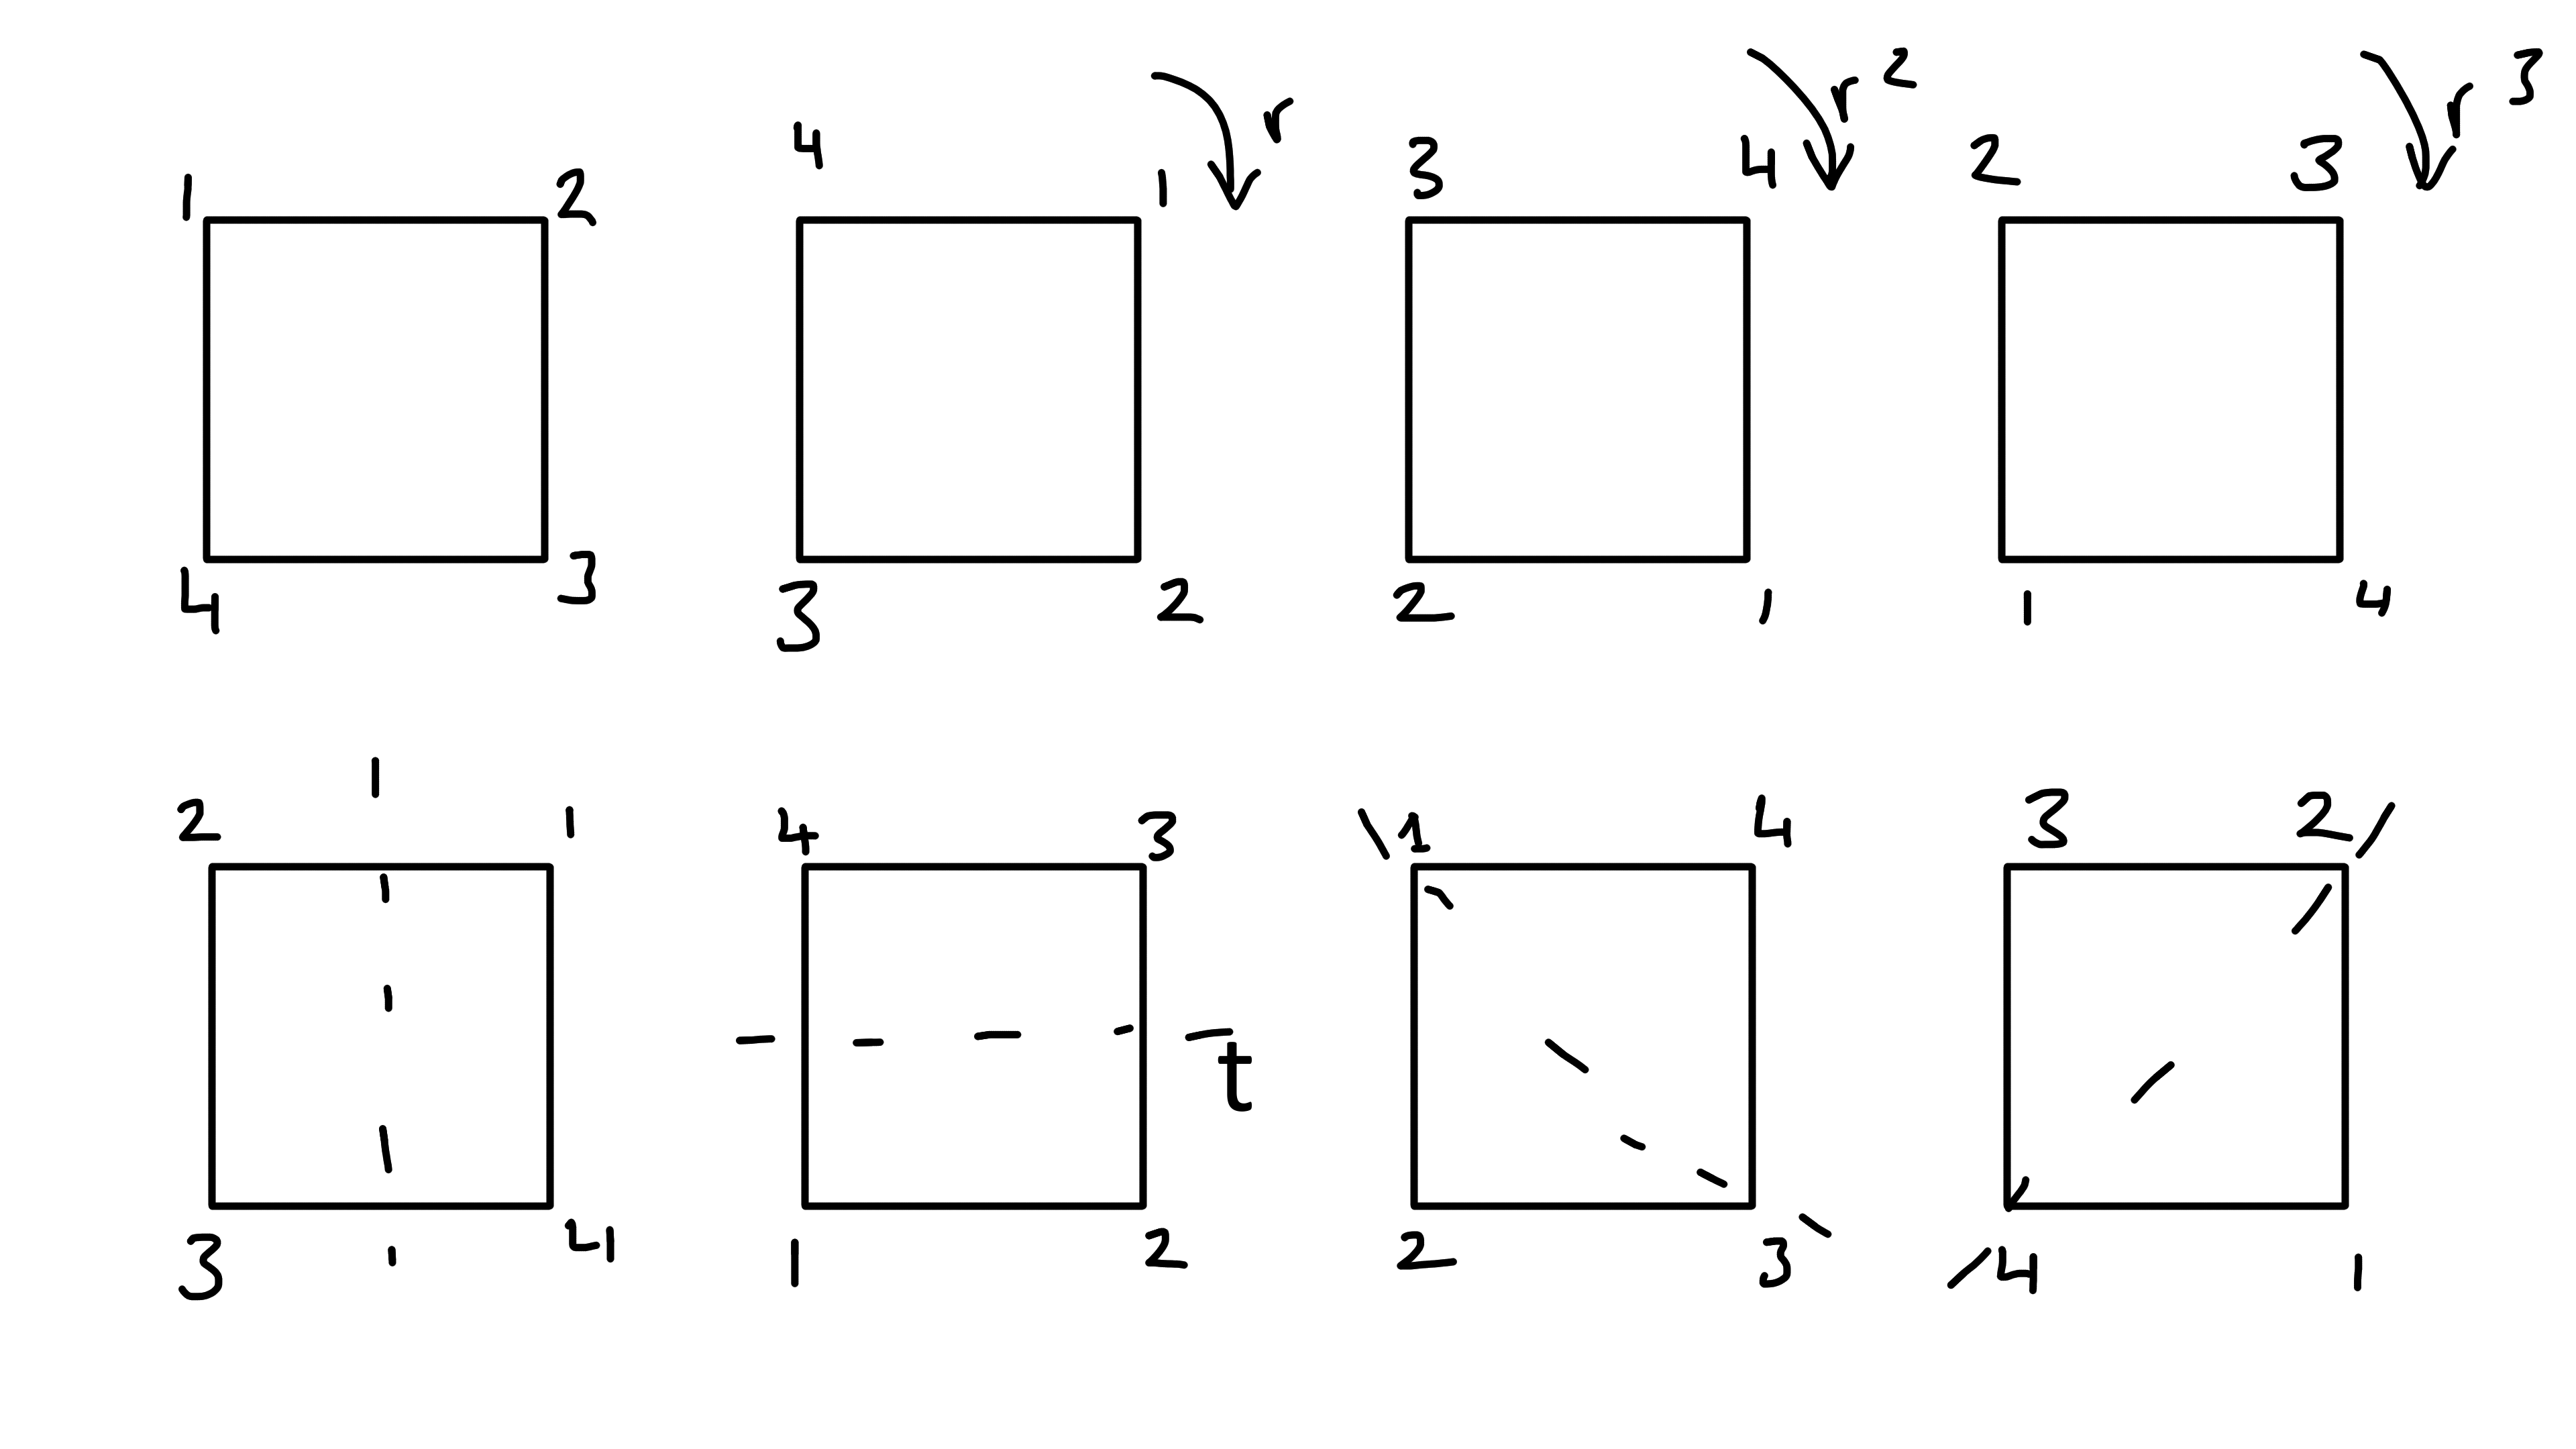
\includegraphics{02-D8}}
\end{figure}

\begin{align*}
    \text{Let } r: P &\to P \\
    z &\mapsto e^{2\pi i / n}z \\
    t : P &\to P \\
    z &\mapsto \overline{z}
  \intertext{These are both isometries}
    |r(z) - r(w)| &= |e^{2\pi i / n}z -e^{2\pi i / n}w| \\
    &= |e^{2\pi i / n}||z - w| \\
    &= |z - w| \\
    |t(z) - t(w)|^2 &= |\overline{z} - \overline{w}|^2 \\
    &=(\overline{z} - \overline{w})(z - w) \\
    &= |z - w|^2 \\
    \implies |t(z) - t(w)| &= |z - w| \\ \\
    \text{Note, } r^n &= \operatorname{id} = \text{identity} \\
    \implies r^{-1} &= r^{n - 1} \\
    t^2 &= \operatorname{id} \\
    \implies t^{-1} &= t \\
    t * r * z &= e^{-2\pi i / n} \ \overline{z} = r^{-1} * t * z \\
    \implies tr &= r^{-1}t
\end{align*}

We show that the set of symmetries of $P$ is precisely $\{e, \underbrace{r, r^2, \dots, r^{n-1}}_\text{rotations}, \underbrace{t, rt \dots, r^{n-1}t}_\text{reflections} \}$.
Then this set under composition of functions gives the group $D_{2n}$.

Let $f$ be a symmetry of $P$. Then $f(1) = e^{2 \pi i k /n}$ for some $k$ ($f(1)$ is mapping $1$ to some vertex, so some element of $V$).
\begin{align*}
    \implies \underbrace{r^{-k} \circ f}_\text{$g$, symmetry of $P$ fixing $1$}(1) &= 1 \\
    g &= r^{-k} \circ f
\end{align*}

So, $g(e^{2 \pi i /n}) = e^{2 \pi i /n}$ or $e^{-2 \pi i /n}$ as the vertices next to $1$ stay next to it.

If $g(e^{2 \pi i /n}) = e^{2 \pi i /n}$ then $g$ fixes the points $1$ and $e^{2 \pi i / n}$.
Also $g$ interchanges the vertices of $P$ so fixes $P$'s centre of mass
\begin{align*}
    \frac{1}{n} \sum_{k=0}^{n-1} e^{2 \pi i k /n} = 0
\end{align*}
So $g$ fixes $0, 1$ and $e^{2 \pi i / n} \implies g = \text{id} \implies f = r^{k}$.

If $g(e^{2 \pi i /n}) = e^{-2 \pi i /n}$ then $t \circ g(e^{2 \pi i / n}) = e^{2 \pi i / n}$
\begin{align*}
    && t \circ g(e^{2 \pi i / n}) &= e^{2 \pi i / n} \\
    && t \circ g (1) &= 1 \\
    && t \circ g (0) &= 0 \\
    &\implies & t \circ g &= \text{id} \\
    &\implies & t \circ r^{-k} \circ f &= \text{id} \\
    &\implies & f &= r^{k} \circ t^{-1} \\
    && &= r^k \circ t
\end{align*}

Algebraically we write,
\begin{align*}
    D_{2n} = \left\langle \underbrace{r,\ t}_\text{generators} | \underbrace{r^n = e,\ t^2 = e,\ trt = r^{-1}}_\text{relations} \right\rangle 
\end{align*}

Finally, $D_2 \cong C_2$ and $D_4$ is \Cref{exm:nine}.
Both are abelian.
Also $D_\infty$ exists.

\hypertarget{symmetric-groups}{%
\subsection{Symmetric Groups}\label{symmetric-groups}}

\begin{definition}[permutation] \label{def:permutation}
Let $X$ be a set.
A bijection \begin{align*}
    f: X \to X
\end{align*} is called a \emph{permutation} of $X$.
Let $\operatorname{Sym} X$ denote the set of all permutations of $X$.
\end{definition} 

\begin{proposition}
$\operatorname{Sym} X$ is a group under composition of functions. It is called the symmetric group on $X$.
\end{proposition}

\begin{proof} ~
\begin{itemize}
\item
  closure - See \Cref{lem:two} (Number's and Sets).
\item
  identity, define $\iota (x) = x \quad \forall \; x \in X$.
\item
  Let $f \in \operatorname{Sym}(X)$.
  As $f$ is a bijection, $f^{-1}$ exists and is a bijection and satisfies $f \circ f^{-1} = \iota = f^{-1} \circ f$.
\item
  composition of functions is associative.
\end{itemize}
\end{proof}

\begin{notation}
Suppose $X$ is finite, $|X| = n$.
Then we often take $X$ to be the set $\{ 1, \dots, n \}$ and we write $S_n$ for $\operatorname{Sym} X$.
We call $S_n$ the symmetric group of degree $n$.
\end{notation}

\begin{notation}[Double row notation]
We'll use double row notation (for now).

If $\sigma \in S_n$ write
\begin{align*}
  G = \begin{pmatrix}
  1 & 2 & \dots & n \\
  \sigma(1) & \sigma(2) & \dots & \sigma(n)
  \end{pmatrix} \\
\end{align*}
\end{notation} 
%
\begin{example} ~\vspace*{-1.5\baselineskip}
  \begin{align*}
    \begin{pmatrix}
    1 & 2 & 3 \\
    2 & 3 & 1
    \end{pmatrix} \in S_3 \\
    \begin{pmatrix}
    1 & 2 & 3 & 4 & 5 \\
    2 & 3 & 1 & 4 & 5
    \end{pmatrix} \in S_5
\end{align*}
\end{example} 

\begin{example}
  Composition:
\begin{align*}
    \begin{pmatrix}
    1 & 2 & 3 \\
    2 & 3 & 1
    \end{pmatrix} \circ
    \begin{pmatrix}
    1 & 2 & 3 \\
    2 & 1 & 3
    \end{pmatrix}
    &= ``\begin{pmatrix}
    1 & 2 & 3 \\
    2 & 1 & 3 \\
    3 & 2 & 1
    \end{pmatrix}" \\
    &= \begin{pmatrix}
        1 & 2 & 3 \\
        3 & 2 & 1
    \end{pmatrix}
\end{align*}
or:

{\centering 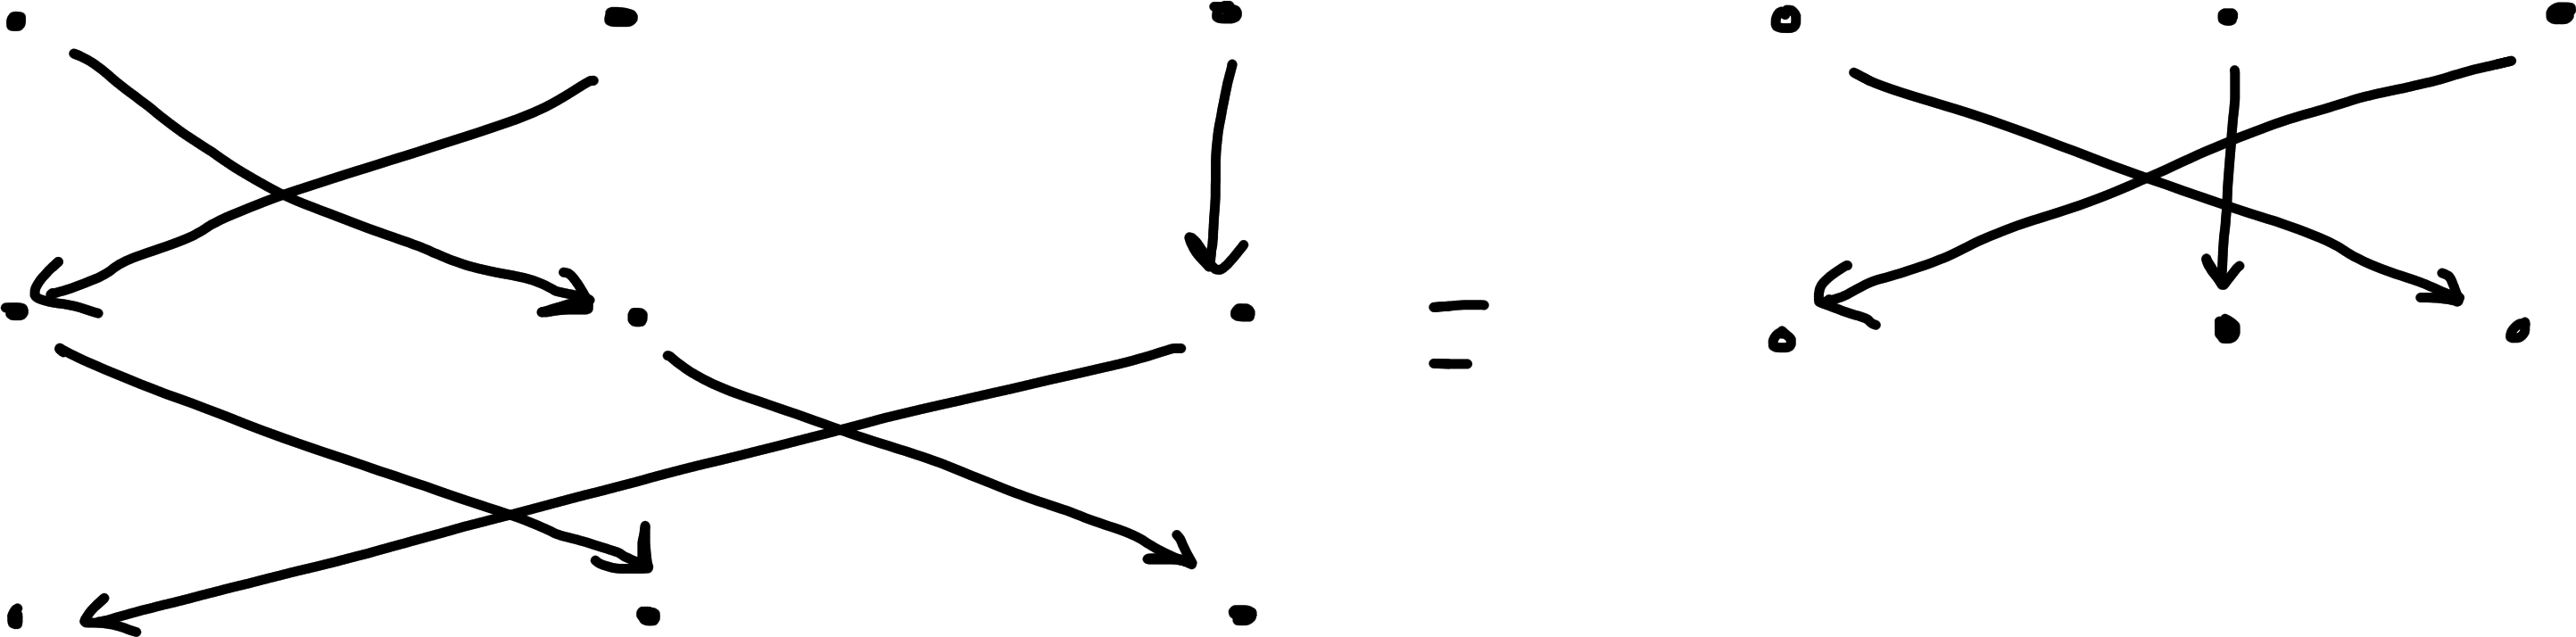
\includegraphics{02-symmetric-graphical}}
\end{example} 

\hypertarget{small-n}{%
\subsubsection{Small n}\label{small-n}}

\begin{example} ~\vspace*{-1.5\baselineskip}
\begin{align*}
  S_1 &= \left\{ \begin{pmatrix}1 \\1\end{pmatrix} \right\} = \{ \iota \} \hspace{.5cm} \text{trivial group} \\
  S_2 &= \left\{ \begin{pmatrix}
  1 & 2 \\
  1 & 2
  \end{pmatrix}, \begin{pmatrix}
  1 & 2 \\
  2 & 1
  \end{pmatrix} \right\} \\
  &\cong \left( \{ \pm 1 \}, \times \right) \cong C_2 \\
  S_3 &= \left\{ \begin{pmatrix}
  1 & 2 & 3 \\
  1 & 2 & 3
  \end{pmatrix}, 
  \begin{pmatrix}
  1 & 2 & 3 \\
  2 & 3 & 1
  \end{pmatrix}, 
  \begin{pmatrix}
      1 & 2 & 3 \\
      3 & 1 & 2
  \end{pmatrix}, 
  \begin{pmatrix}
      1 & 2 & 3 \\
      1 & 3 & 2
  \end{pmatrix}, 
  \begin{pmatrix}
      1 & 2 & 3 \\
      3 & 2 & 1
  \end{pmatrix}, 
  \begin{pmatrix}
      1 & 2 & 3 \\
      2 & 1 & 3
  \end{pmatrix} \right\} \\
  & \cong D_6
\end{align*}
\end{example} 

\begin{remark} ~
\begin{enumerate}
\def\labelenumi{\roman{enumi}.}
\item
  $|S_n| = n!$
\item
  For $n \geq 3$ $S_n$ is not abelian.
  Consider
  \begin{align*}
  \begin{pmatrix}
  1 & 2 & 3 & 4 & \dots & n \\
  2 & 3 & 1 & 4 & \dots & n
  \end{pmatrix}, 
  \begin{pmatrix}
      1 & 2 & 3 & 4 & \dots & n \\
      1 & 3 & 2 & 4 & \dots & n
  \end{pmatrix}
  \end{align*}
  They don't commute in $S_3$ so they won't in $S_n$.
\item
  $D_{2n}$ naturally embeds in $S_n$.
  e.g.~$D_8 \lesssim S_4$ (isomorphic to a subgroup)
  \begin{align*}
      r = \begin{pmatrix}
      1 & 2 & 3 & 4 \\
      2 & 3 & 4 & 1
      \end{pmatrix},\ t = 
      \begin{pmatrix}
      1 & 2 & 3 & 4 \\
      4 & 3 & 2 & 1
      \end{pmatrix}
  \end{align*}
\end{enumerate}

\end{remark}

`Double row notation is cumbersome and hides what's going on, so we introduce cycle notation'.

\begin{definition}[Cycle notation]
Let $a_1, \dots, a_k$ be distinct integers in $\{ 1, \dots, n \}$.
Suppose $\sigma \in S_n$ and
\begin{align*}
    \sigma(a_i) &= a_{i + 1} \hspace{0.5cm} 1 \leq 1 \leq k - 1 \\
    \sigma(a_k) &= a_1
\end{align*}
and $\sigma(x) = x \; \forall \; x \in \{ 1, \dots, n \} \setminus \{ a_1, \dots, a_k \}$.
Then $\sigma$ is a \emph{k-cycle} and we write $\sigma = (a_1, a_2, \dots, a_k)$.
e.g.~\begin{align*}
    \sigma = \begin{pmatrix}
    1 & 2 & 3 \\
    2 & 3 & 1
    \end{pmatrix}
\end{align*} is the 3-cycle $\begin{pmatrix}1 & 2 & 3\end{pmatrix}$ i.e. $1 \mapsto 2$, $2\mapsto 3$, $3\mapsto 1$ and all of numbers map to themselves.
\end{definition}

\begin{remark} ~
\begin{enumerate}
\def\labelenumi{\roman{enumi}.}
\item
  \begin{align*}
   (a_1, a_2, \dots, a_k) &= (a_k, a_1, a_2, \dots, a_{k-1}) \\
   &= \dots
  \end{align*} We usually write the smallest $a_i$ first.
\item
  \begin{align*}
  (a_1, a_2, \dots, a_k)^{-1} &= (a_1, a_k, a_{k-1}, \dots, a_2).
  \end{align*}
\item
  $o(\sigma) = k$, $\sigma$ is like the rotations of k points.
  \begin{figure}
    \centering 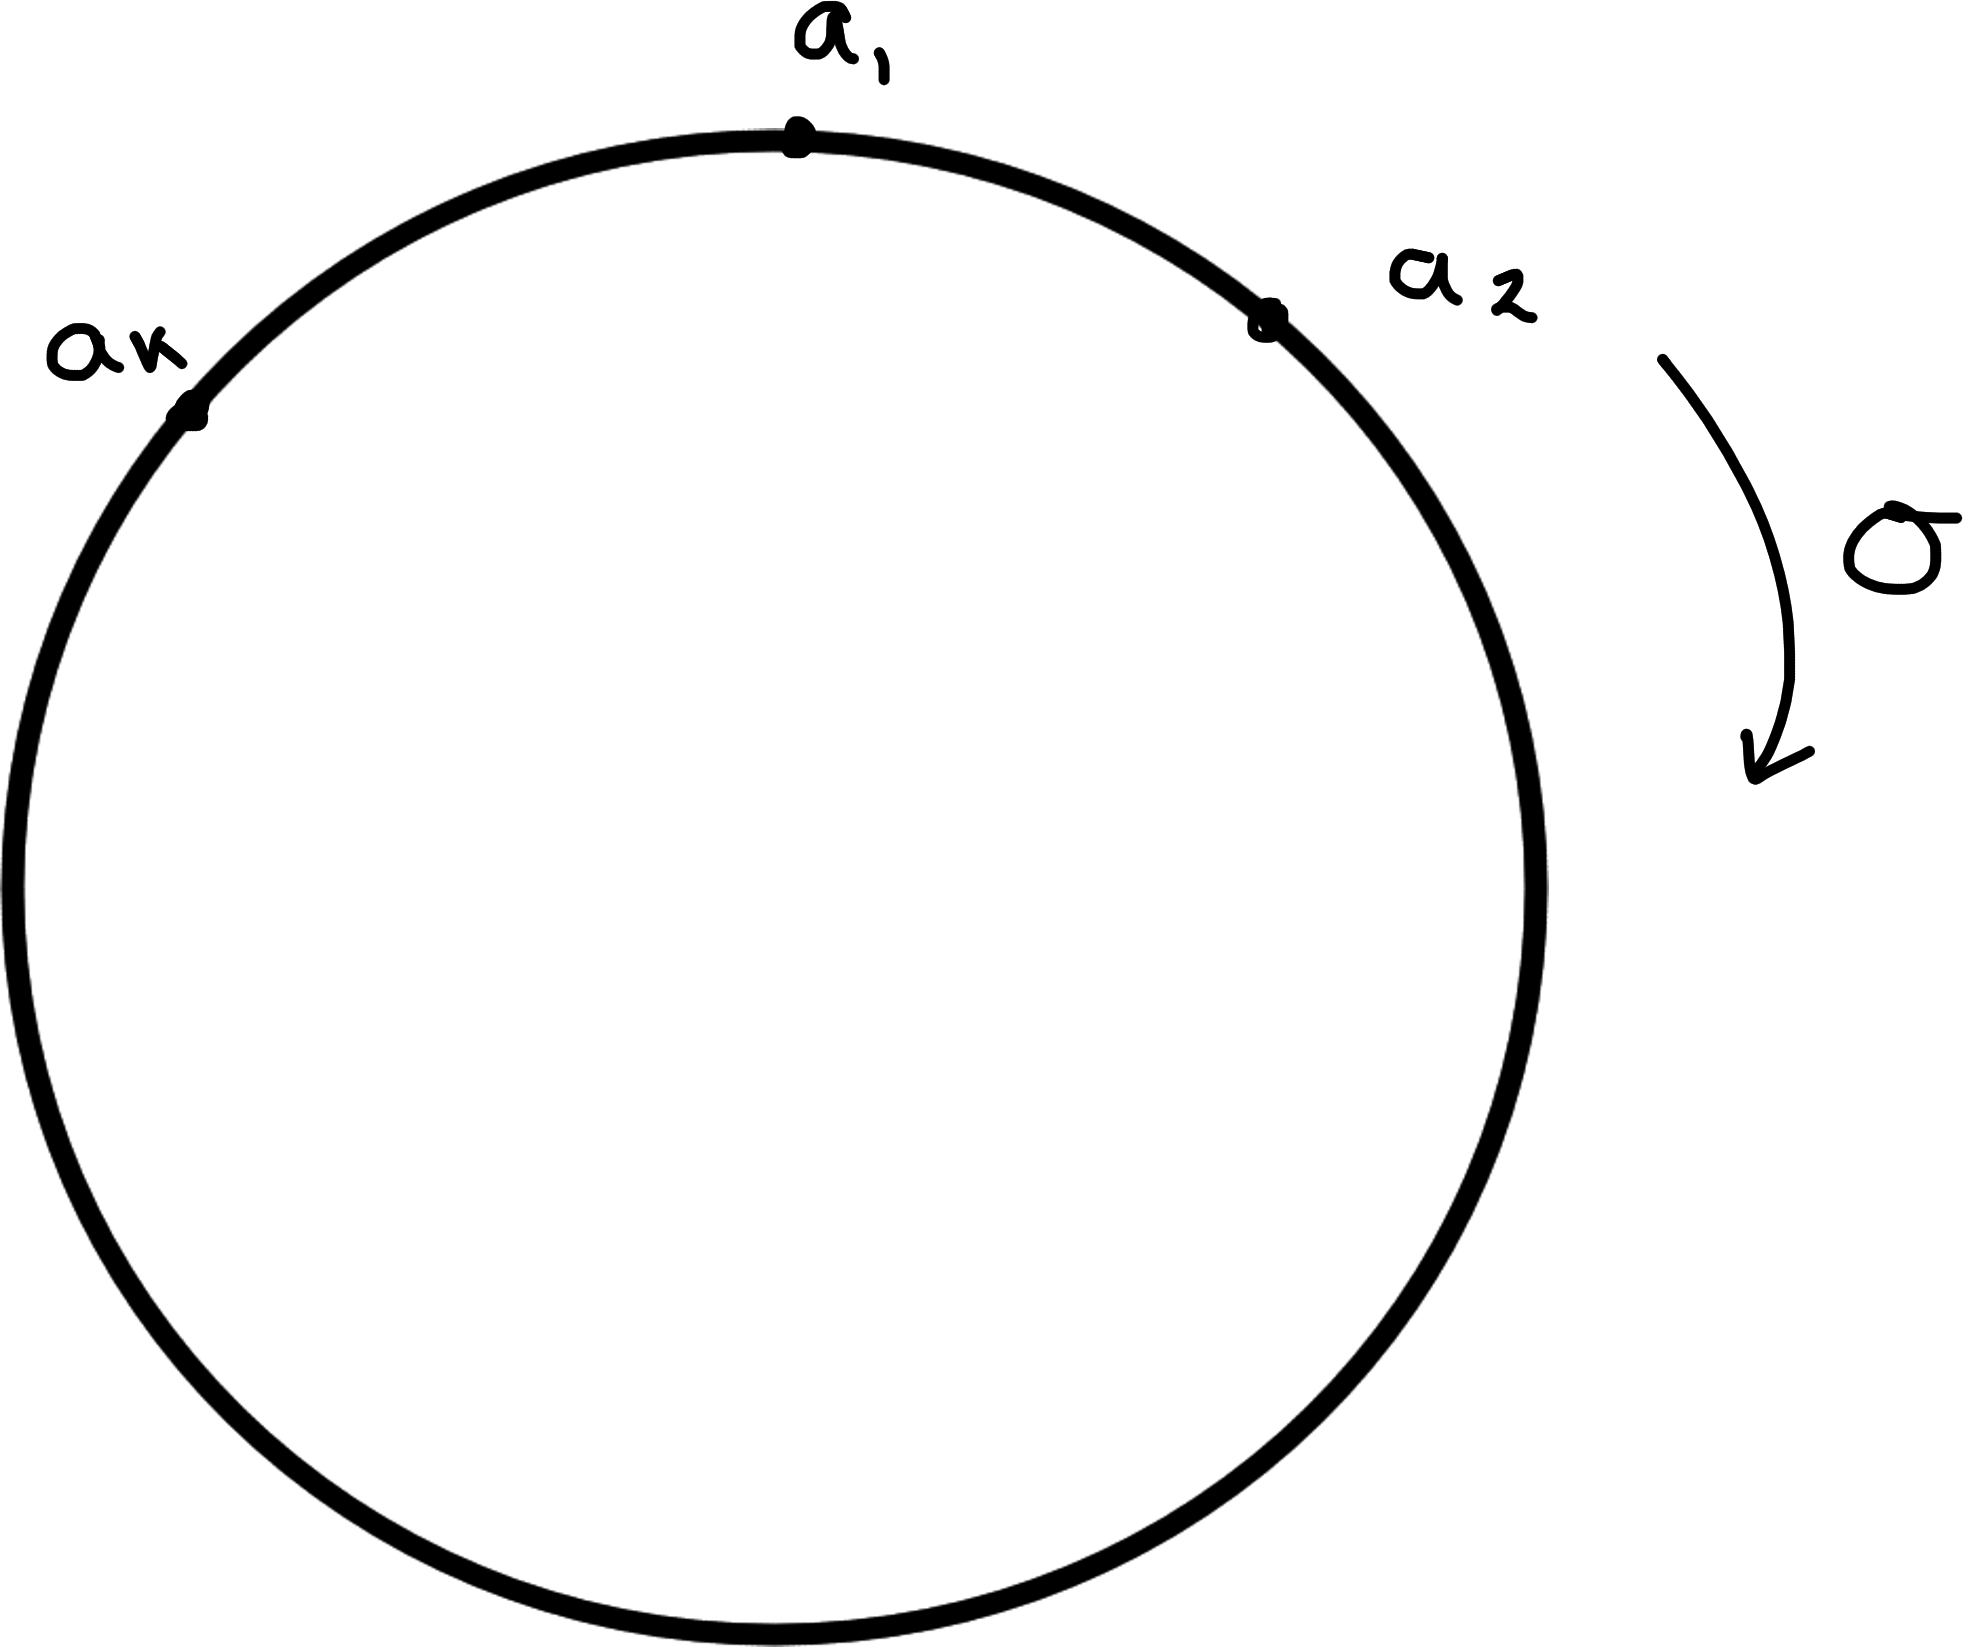
\includegraphics[width=0.5\linewidth]{02-sigma-graphical}
  \end{figure} 
\item
  a 2-cycle is called a \emph{transposition}.
\end{enumerate}

\end{remark}

\begin{definition}[Disjoint cycles]
Two cycles $\sigma = (a_1, \dots, a_k)$ and $\tau = (b_1, \dots, b_l)$ are \emph{disjoint} if $\{ a_1, \dots, a_k \} \cap \{ b_1, \dots, b_k \} = \emptyset$.
\end{definition}

\begin{lemma}
\protect\hypertarget{lem:six}{}\label{lem:six}
If $\sigma, \tau \in S_n$ are disjoint then $\sigma \tau = \tau \sigma$
\end{lemma}

\begin{proof}
If $x \in {1, \dots, n} \setminus \{ a_1, \dots, a_k \} \cup \{ b_1, \dots, b_k \}$, $(\sigma \circ \tau) (x) = \sigma \left( \tau(x) \right) = (\tau \circ \sigma)(x)$.

Suppose $1 \leq i \leq k - 1$
\begin{align*}
    (\sigma \circ \tau)(a_i) &= \sigma\left(\tau(a_i) \right) \\
    &= \sigma(a_i) = a_{i + 1} \\
    (\tau \circ \sigma)(a_i) &= \tau\left(\sigma(a_i) \right) \\
    &= \tau(a_{i + 1}) = a_{i + 1}
\end{align*}
And $\sigma \circ \tau (a_k) = a_1$, $\tau \circ \sigma (a_k) = a_1$.

Similarly for $b_j$
$\tau \circ \sigma (b_j) = \sigma \circ \tau (b_j)$

Thus $\sigma \circ \tau$ and $\tau \circ \sigma$ agree everywhere $\implies \sigma \circ \tau = \tau \circ \sigma$.
\end{proof}

\begin{example}
$\begin{pmatrix}1 & 2\end{pmatrix} \begin{pmatrix}3 & 4 & 5\end{pmatrix} = \begin{pmatrix}3 & 4 & 5\end{pmatrix} \begin{pmatrix}1 & 2\end{pmatrix}$
\end{example}

However this is not necessarily true if two cycles are not disjoint.

\begin{example} ~\vspace*{-1.5\baselineskip}
\begin{align*}
    \sigma = \begin{pmatrix}1 & 2 & 3\end{pmatrix},\ \tau &= \begin{pmatrix}2 & 4\end{pmatrix} \\
    \sigma \circ \tau(1) &= \sigma(1) = 2 \\
    \sigma \circ \tau(2) &= \sigma(4) = 4 \\
    \sigma \circ \tau(3) &= \sigma(3) = 1 \\
    \sigma \circ \tau(4) &= \sigma(2) = 3 \\
    \sigma \circ \tau &= \begin{pmatrix}1 & 2 & 4 & 3\end{pmatrix} \\
    \text{But } \tau \circ \sigma &= \begin{pmatrix} 1 & 4 & 2 & 3 \end{pmatrix}
\end{align*}
\end{example}

\begin{example} ~\vspace*{-1.5\baselineskip}
\begin{align*}
    \begin{pmatrix}1 & 2 & 3\end{pmatrix} \begin{pmatrix}2 & 3\end{pmatrix} &= \begin{pmatrix}1 & 2\end{pmatrix} \begin{pmatrix} 3 \end{pmatrix} \\
    &= \begin{pmatrix}1 & 2\end{pmatrix} \text{ suppress 1-cycles.} \\
    \begin{pmatrix}2 & 3\end{pmatrix} \begin{pmatrix}1 & 2 & 3\end{pmatrix} &= \begin{pmatrix}1 & 3\end{pmatrix} 
\end{align*}
\end{example}

\begin{theorem}
\protect\hypertarget{thm:one}{}\label{thm:one}Every permutation can be written as a product of disjoint cycles (in an essentially unique way).
\end{theorem}

\begin{example} ~\vspace*{-1.5\baselineskip}
\begin{align*}
    \sigma &= \begin{pmatrix}
    1 & 2 & 3 & 4 & 5 & 6 & 7 & 8 & 9 \\
    2 & 4 & 5 & 7 & 6 & 3 & 1 & 9 & 8
    \end{pmatrix} \\
    &= \begin{pmatrix} 1 & 2 & 4 & 7 \end{pmatrix} \begin{pmatrix}3 & 5 & 6\end{pmatrix} \begin{pmatrix}8 & 9\end{pmatrix}
\end{align*}
\end{example}

\begin{proof}
Let $a_1 \in \{ 1, 2, \dots, n \} = X$.
Consider $a_1, \sigma(a_1), \sigma^2(a_1), \dots$\\
Since $X$ is finite $\exists$ minimal $j$ such that $\sigma^j(a_1) \in \{ a_1, \sigma(a_1), \sigma^2(a_1), \dots, \sigma^{j-1}(a_1) \}$.
We claim: $\sigma^j(a_1) = a_1$.
Since if not \begin{align*}
    \sigma^j(a_1) &= \sigma^i(a_1),\ j > i \geq 1 \\
    \implies \sigma^{j - i}(a_1) &= a_1 \quad \text{\Lightning \ of minimality of j.}
\end{align*}
So $\{ a_1, \sigma(a_1), \sigma^2(a_1), \dots, \sigma^{j-1}(a_1) \}$ is a cycle in $\sigma$.\\
If $\exists \; b \in X \setminus \{ a_1, \sigma(a_1), \sigma^2(a_1), \dots, \sigma^{j-1}(a_1) \}$.
Consider $b, \sigma(b), \dots$\\
Note $\left(b, \sigma(b), \sigma^2(b), \dots, \sigma^{j-1}(b) \right)$ is disjoint from $\left( a_1, \sigma(a_1), \sigma^2(a_1), \dots, \sigma^{j-1}(a_1) \right)$ because $\sigma$ is a bijection.\footnote{If $\sigma^i(b) = \sigma^j(a_1)$ then $b = \sigma^{j - i}(a_1)$ which contradicts $b \in X \setminus \{ a_1, \sigma(a_1), \sigma^2(a_1), \dots, \sigma^{j-1}(a_1) \}$.}\\
Continue in this way until all elements of $X$ are reached.
\end{proof}

\begin{lemma}
Let $\sigma, \tau$ be disjoint cycles in $S_n$.
Then $o(\sigma \tau) = \operatorname{lcm} \{ o(\sigma), o(\tau) \}$
\end{lemma}

\begin{proof}
Let $k = \operatorname{lcm} \{ o(\sigma), o(\tau) \}$ so $o(\sigma) \mid k$ and $o(\tau) \mid k$.
Then \begin{align}
    (\sigma \tau)^k &= \sigma \tau \sigma \tau \dots \sigma \tau \notag\\
    &= \sigma^k \tau^k \quad \text{\Cref{lem:six}} \notag \\
    &= e \cdot e \quad \text{\Cref{lem:five}} \notag\\
    &= e \notag \\
    \implies o(\sigma \tau) \mkern-5mu &\;\mid k \quad \text{\Cref{lem:five}} \label{lem:2.2-proof}
\end{align}
Now suppose $o(\sigma \tau) = n$ so $(\sigma \tau)^n = e \implies \sigma^n \tau^n = e$.
But $\sigma, \tau$ move different elements of $X \implies \sigma^n = e,\ \tau^n = e$.
By \Cref{lem:five}
\begin{align}
    \implies o(\sigma) \mkern-5mu &\;\mid n \text{ and } o(\tau) \mid n \notag\\
    \implies k &= \operatorname{lcm} \{ o(\sigma), o(\tau) \} \notag\\
    &\;\mid n = o(\sigma \tau) \label{lem:2.2-proof2} \\
    \cref{lem:2.2-proof},\ \cref{lem:2.2-proof2} \implies o(\sigma \tau) &= \operatorname{lcm} \{ o(\sigma), o(\tau) \} \notag
\end{align}
\end{proof}

\begin{proposition}
Any $\sigma \in S_n \ (n \geq 2)$ can be written as a product of transpositions.
\end{proposition}

\begin{proof}
By \Cref{thm:one} it is enough to show a k-cycle can be written as a product of transpositions.
\begin{align*}
    \begin{pmatrix}a_1 & a_2 & \dots & a_k \end{pmatrix}
    &= \begin{pmatrix}a_1 & a_2\end{pmatrix} \begin{pmatrix}a_2 & a_3\end{pmatrix} \dots \begin{pmatrix}a_{k-2} & a_{k-1}\end{pmatrix} \begin{pmatrix}a_{k-1} & a_k\end{pmatrix}
\end{align*}
\end{proof}

\begin{example} ~\vspace*{-1.5\baselineskip}
\begin{align*}
    \begin{pmatrix}1 & 2 & 3 & 4 & 5\end{pmatrix} &= \begin{pmatrix}1 & 2\end{pmatrix} \begin{pmatrix}2 & 3\end{pmatrix} \begin{pmatrix}3 & 4\end{pmatrix} \begin{pmatrix}4 & 5\end{pmatrix} \\
    &= \begin{pmatrix}1 & 2\end{pmatrix} \begin{pmatrix}1 & 2\end{pmatrix} \begin{pmatrix}1 & 2\end{pmatrix} \begin{pmatrix}2 & 3\end{pmatrix} \begin{pmatrix}3 & 4\end{pmatrix} \begin{pmatrix}4 & 5\end{pmatrix} \\
    &= \begin{pmatrix}1 & 5\end{pmatrix} \begin{pmatrix}1 & 4\end{pmatrix} \begin{pmatrix}1 & 3\end{pmatrix} \begin{pmatrix}1 & 2\end{pmatrix}
\end{align*}
\emph{not unique}.
\end{example}

\begin{definition}[Sign of permutation]
Let $\sigma \in S_n \ (n \geq 2)$.
Then the \emph{sign} of $\sigma$, written $\operatorname{sgn}(\sigma)$, is $(-1)^k$ is the number of transpositions in some expression of $\sigma$ as a product of transpositions.
\end{definition}

\begin{lemma}
\protect\hypertarget{lem:eight}{}\label{lem:eight}The function \begin{align*}
    \operatorname{sgn} : S_n &\to \{ \pm 1 \} \\
    \sigma &\mapsto \operatorname{sgn}(\sigma)
\end{align*} is well defined.\\
i.e.~if $\sigma = \tau_1 \dots \tau_a = \tau_1' \dots \tau_b'$ with $\tau_i$ and $\tau_i'$ transpositions then $(-1)^a = (-1)^b$.
\begin{align*}
    \operatorname{sgn}\left(\begin{pmatrix}1 & 2 & 3 & 4 & 5\end{pmatrix}\right) &= (-1)^4 = (-1)^6 \\
    &= 1
\end{align*}
\end{lemma}

\begin{proof}
Let $c(\sigma)$ denote the number of cycles in a disjoint cycle decomposition of $\sigma$ including 1-cycles, so $c(\text{id}) = n$.\\
Let $\tau$ be a transposition.
Claim: $c(\sigma \tau) = c(\sigma) \pm 1 \equiv c(\sigma) + 1 \mod 2$.\\
Let $\tau = \begin{pmatrix}k & l\end{pmatrix}$.\\
2 cases:

\begin{enumerate}
\def\labelenumi{\roman{enumi}.}
\item
  $k, l$ lie in different cycles of $\sigma$:
  \begin{align*}
   \begin{pmatrix}k & a_1 & \dots & a_r \end{pmatrix} \begin{pmatrix}l & b_1 & \dots & b_s \end{pmatrix} \begin{pmatrix} k & l\end{pmatrix}
   &= \begin{pmatrix}k & b_1 & b_2 & \dots & b_s & l & a_1 & \dots & a_r \end{pmatrix} \\
   \implies c(\sigma \tau) &= c(\sigma) - 1
  \end{align*}
\item
  \begin{enumerate}
  \def\labelenumii{\roman{enumii}.}
  \tightlist
  \item
    $k, l$ lie in the same cycle in $\sigma$:
    \begin{align*}
    \begin{pmatrix}k & a_1 & \dots & a_r & l & b_1 & \dots & b_s \end{pmatrix} \begin{pmatrix} k & l\end{pmatrix}
    &= \begin{pmatrix}k & b_1 & b_2 & \dots & b_s \end{pmatrix} \begin{pmatrix}l & a_1 & \dots & a_r \end{pmatrix} \\
    \implies c(\sigma \tau) &= c(\sigma) + 1
    \end{align*}
  \end{enumerate}
\end{enumerate}

Assume \begin{align*}
    \sigma &= \text{id} \tau_1 \dots \tau_a \\
    &= \text{id} \tau_1' \dots \tau_b' \\
    \implies c(\sigma) &\equiv n + a \mod 2 \\
    &\equiv n + b \mod 2 \\
    \implies a &\equiv b \mod 2 \\
    \implies (-1)^a &= (-1)^b
\end{align*}
\end{proof}


\begin{aside}{Aside: Subgroup Lattices}
Subgroup lattice of $D_6 = \{ e, r, r^2, t, rt, r^2t \}$

\begin{center}
  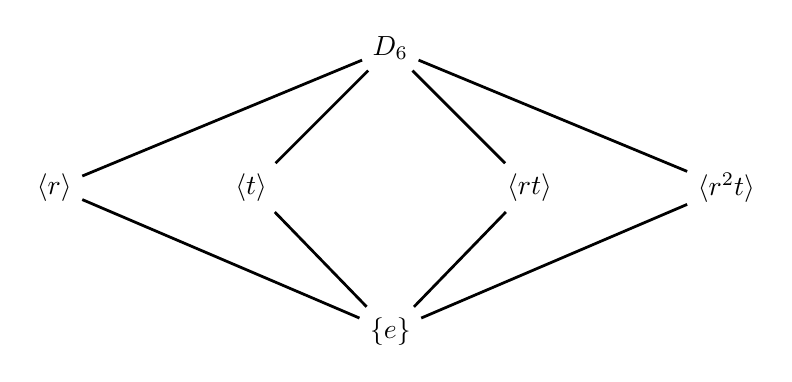
\begin{tikzpicture}[node distance=2.5cm, line width=1pt]
    \node(A4) at (0,0)     {$D_6$};
    \node(C32)      [below left of=A4]       {$\langle t \rangle$};
    \node(C31)      [left of=C32]  {$\langle r \rangle$};
    \node(C33)      [below right of=A4]       {$\langle rt \rangle$};
    \node(C34)      [right of=C33]       {$\langle r^2t \rangle$};
    
    \node(1)        [below=3cm,at=(A4.south)]   {$\left\{e\right\}$};
    \draw(A4)       -- (C31);
    \draw(A4)       -- (C32);
    \draw(A4)       -- (C33);
    \draw(A4)       -- (C34);
    \draw(C31)      --  (1);
    \draw(C32)      --  (1);
    \draw(C33)      --  (1);
    \draw(C34)      --  (1);
  \end{tikzpicture}   
\end{center}

We put the largest subgroups at the top and work our way down.

\end{aside}

\begin{theorem}
\protect\hypertarget{thm:two}{}\label{thm:two}Let $n \geq 2$.
The map
\begin{align*}
    \operatorname{sgn} : (S_n, \circ) &\to \left( \{ \pm 1 \}, \times \right) \\
    \sigma *\mapsto \operatorname{sgn}(\sigma)
\end{align*}
is a well-defined non-trivial (doesn't just map to identity) homomorphism.
\end{theorem}

\begin{proof}
~

\begin{itemize}
\item
  We know its well-defined by \Cref{lem:eight}
\item
  $\operatorname{sgn}\left( \begin{pmatrix}1 & 2\end{pmatrix} \right) = -1$, so non-trivial
\item
  homomorphism:
\end{itemize}

Let $\alpha, \beta \in S_n$ with $\operatorname{sgn} (\alpha) = (-1)^k$, $\operatorname{sgn} (\alpha) = (-1)$.
So $\exists$ transpositions $\tau_i$ and $\tau_i'$ such that $\alpha = \tau_1 \dots \tau_k$ and $\beta = \tau_1' \dots \tau_l'$.
This implies
\begin{align*}
    \alpha \beta &= \tau_1 \dots \tau_k \tau_1' \dots \tau_l' \\
    \implies \operatorname{sgn}(\alpha \beta) &= (-1)^{k + l} \\
    &= (-1)^k (-1)^l \\
    &= \operatorname{sgn}(\alpha) \operatorname{sgn}(\beta)
\end{align*}
\end{proof}

\begin{definition}
\protect\hypertarget{def:eleven}{}\label{def:eleven}
$\sigma$ is an \emph{even} permutation if $\operatorname{sgn}(\sigma) = 1$ and an odd permutation if $\operatorname{sgn}(\sigma) = -1$.
\end{definition}

\begin{corollary}
The even permutations of $S_n$ ($n \geq 2$) form a subgroup called the \emph{alternating group} and we denote it by $A_n$.
\end{corollary}

\begin{proof} ~

\begin{itemize}
  \item id $= \begin{pmatrix}1 & 2\end{pmatrix} \begin{pmatrix}1 & 2\end{pmatrix} \in A_n$

  \item
    \begin{align*}
      \operatorname{sgn}(\sigma) &= 1 = \operatorname{sgn}(\rho) \\ 
      \implies \operatorname{sgn}(\sigma \rho) &= \operatorname{sgn}(\sigma) \operatorname{sgn}(\rho) \\
      &= 1
    \end{align*} by Theorem \ref{thm:two}
  \item
    $\sigma = \tau_1 \dots \tau_k$ where $\tau_i$ are transpositions.
    Then $\sigma^{-1} = \tau_k \dots \tau_1 \implies \operatorname{sgn}(\sigma) = \operatorname{sgn}(\sigma^{-1})$
  \item
    associativity is inherited
\end{itemize}

\end{proof}

\begin{example}
$A_4 = \{ e, \begin{pmatrix}1 & 2\end{pmatrix} \begin{pmatrix}3 & 4\end{pmatrix}, \begin{pmatrix}1 & 3\end{pmatrix} \begin{pmatrix}2 & 4\end{pmatrix}, \begin{pmatrix}1 & 4\end{pmatrix} \begin{pmatrix}2 & 3\end{pmatrix},\begin{pmatrix}1 & 2 & 3\end{pmatrix}, \begin{pmatrix}1 & 3 & 2\end{pmatrix},$ \\
$\begin{pmatrix}1 & 2 & 4\end{pmatrix}, \begin{pmatrix}1 & 4 & 2\end{pmatrix},\begin{pmatrix}2 & 3 & 4\end{pmatrix}, \begin{pmatrix}2 & 4 & 3\end{pmatrix}, \begin{pmatrix}1 & 3 & 4\end{pmatrix}, \begin{pmatrix}1 & 4 & 3\end{pmatrix} \}$.
\end{example}

\begin{remark} ~
  \begin{enumerate}
  \def\labelenumi{\roman{enumi}.}
  \item
    $|A_n| = \frac{|S_n|}{2} = \frac{n!}{2}$ (will be proved later on)
  \item
    cycles of even length are odd and cycles of odd length are even.
  \item
    $A_n = \ker (\text{sgn})$, hence a subgroup (q9 - sheet 1).
  \end{enumerate}
\end{remark}